\documentclass{IEEEtaes}


\usepackage[colorlinks,urlcolor=blue,linkcolor=blue,citecolor=blue]{hyperref}

\usepackage{color,array,amsthm}

\usepackage{graphicx}

\jvol{XX}
\jnum{XX}
\jmonth{XXXXX}
\paper{1234567}
\pubyear{2020}
\doiinfo{TAES.2020.Doi Number}

\newtheorem{theorem}{Theorem}
\newtheorem{lemma}{Lemma}
\setcounter{page}{1}
%% \setcounter{secnumdepth}{0}



\begin{document}


\title{Preparation of Articles for IEEE Transactions and Journals (2021)} 


\author{FIRST A. AUTHOR}
\member{Fellow, IEEE}
\affil{National Institute of Standards and Technology, Boulder, CO} 

\author{SECOND B. AUTHOR}
\affil{Colorado State University, Fort Collins, CO 80523, USA} 

\author{THIRD C. AUTHOR Jr.}
\member{Member, IEEE}
\affil{University of Colorado, Boulder, CO 80309, USA}

%% \author{FOURTH D. AUTHOR}
%% \affil{University of Colorado, Colorado, USA}

\receiveddate{This paragraph of the first footnote will contain the date on which you submitted your paper for review, which is populated by IEEE. It is IEEE style to display support information, including sponsor and financial support acknowledgment, here and not in an acknowledgment section at the end of the article. For example, ``This work was supported in part by the U.S. Department of Commerce under Grant BS123456.'' }
%% \accepteddate{XXXXX XX XXXX}
%% \publisheddate{XXXXX XX XXXX}

\corresp{The name of the corresponding author appears after the financial information, e.g. {\itshape (Corresponding author: M. Smith)}. Here you may also indicate if authors contributed equally or if there are co-first authors.}

\authoraddress{The next few paragraphs should contain the authors' current affiliations, including current address and e-mail. For example, First A. Author is with the National Institute of Standards and Technology, Boulder, CO 80305 USA (e-mail: author@ boulder.nist.gov). Second B. Author, Jr., was with Rice University, Houston, TX 77005 USA. He is now with the Department of Physics, Colorado State University, Fort Collins, CO 80523 USA (e-mail: author@lamar.colostate.edu). Third C. Author is with the Electrical Engineering Department, University of Colorado, Boulder, CO 80309 USA, on leave from the National Research Institute for Metals, Tsukuba 305-0047, Japan (e-mail: author@nrim.go.jp).}

\editor{Mentions of supplemental materials and animal/human rights statements can be included here.}
\supplementary{Color versions of one or more of the figures in this article are available online at {http://ieeexplore.ieee.org}.}


\markboth{AUTHOR ET AL.}{SHORT ARTICLE TITLE}
\maketitle


\begin{abstract}This document provides a guide for preparing articles for IEEE Transactions, Journals, and Letters. Use this document as a template if you are using Microsoft {\itshape Word}. Otherwise, use this as an instruction set. The electronic file of your article will be formatted further at IEEE. Titles should be written in uppercase and lowercase letters, not all uppercase. Avoid writing long formulas with subscripts in the title; short formulas that identify the elements are fine (e.g., ``Nd--Fe--B''). Do not write ``(Invited)'' in the title. Full names of authors are preferred in the author field but are not required. Put a space between authors' initials. ORCIDs can be provided here as well. In the title, all variables should appear lightface italic; numbers and units will remain bold. Abstracts must be a single paragraph. In order for an Abstract to be effective when displayed in IEEE {\bfseries\itshape Xplore} as well as through indexing services such as Compendex, INSPEC, Medline, ProQuest, and Web of Science, it must be an accurate, stand-alone reflection of the contents of the article. They shall not contain displayed mathematical equations, numbered reference citations, nor footnotes. They should include three or four different keywords or phrases, as this will help readers to find it. It is important to avoid over-repetition of such phrases as this can result in a page being rejected by search engines. Ensure that your abstract reads well and is grammatically correct.
\end{abstract}

\begin{IEEEkeywords}Enter keywords or phrases in alphabetical order, separated by commas. For a list of suggested keywords, send a blank e-mail to keywords@ieee.org or visit {http://www.ieee.org/organizations/pubs/ani\_prod/keywrd98.txt}
\end{IEEEkeywords}

\section{INTRODUCTION}
T{\scshape his} document is a template for Microsoft {\it Word}. If you would prefer to use LaTeX, download IEEE's LaTeX style and sample files from {https://template-selector.ieee.org/secure/templateSelector/publicationType}. You can also use the Overleaf editor at {https://\break www.overleaf.com/blog/278-how-to-use-overleaf-with-\break ieee-collabratec-your-quick-guide-to-getting-started\#.\break Vp6tpPkrKM9}.

This template is a guide to formatting; your proof and final published version may vary in layout and length to conform to IEEE policy and style. Page count is an estimate; the length of your submitted article in the template may not be the same as when the formal proof is created by IEEE

The {\it IEEE Editorial Style Manual for Authors} is available at {https://journals.ieeeauthorcenter.ieee.org/create-your-ieee-journal-article/create-the-text-of-your-article/ieee-editorial-style-manual/}. This contains a formal set of editorial guidelines for IEEE Transactions, Journals, and Letters, including:
\begin{itemize}
\item punctuation;
\item capitalization;
\item abbreviations;
\item section headings;
\item numbers, equations;
\item footnotes;
\item biographies;
\item some common mistakes;
\item units of measurement.
\end{itemize}

Communicate your work clearly. If you are not fully proficient in English, consider using an English language editing service before submitting your article. An expert editing service can help you refine the use of English in your article, so you can communicate your work more effectively.

The use of an editing service is paid for by the author. It does not guarantee acceptance in an IEEE publication. For more information, visit the IEEE Author Center at {https://journals.ieeeauthorcenter.ieee.org/create-your-ieee-journal-article/create-the-text-of-your-article/structure-your-article/\#editing-service}.

\section{GUIDELINES FOR MANUSCRIPT PREPARATION}

When you open the template, select ``Page Layout'' from the ``View'' menu in the menu bar (View | Page Layout), (these instructions assume Microsoft {\it Word}. Some versions may have alternate ways to access the same functionalities noted here). Then, type over sections of the template or cut and paste from another document and use markup styles. The pull-down style menu is in the Formatting Toolbar at the top of your {\it Word} window (e.g., the style at this point in the document is ``Text''). Highlight a section that you want to designate with a certain style, and then select the appropriate name on the style menu. The style will adjust your fonts and line spacing. Do not change the font sizes or line spacing to squeeze more text into a limited number of pages. Use {\it italics} for emphasis; do not underline.

IEEE will do the final formatting of your article. If your article is intended for a conference, please observe the conference page limits.

This is intended as an authoring template, not a final production template. It is not intended to match the final published format. Differences in final formatting are likely in the final IEEE files. Page count in the template is an estimate. Do not adjust line and character spacing to fit your paper to a specific length.

\subsection{Abbreviations and Acronyms}

Define abbreviations and acronyms the first time they are used in the text, even after they have already been defined in the abstract. Abbreviations such as IEEE, SI, ac, and dc do not have to be defined. Abbreviations that incorporate periods should not have spaces: write ``C.N.R.S.,'' not ``C. N. R. S.'' Do not use abbreviations in the title unless they are unavoidable (for example, ``IEEE'' in the title of this article).

\begin{figure}
\centerline{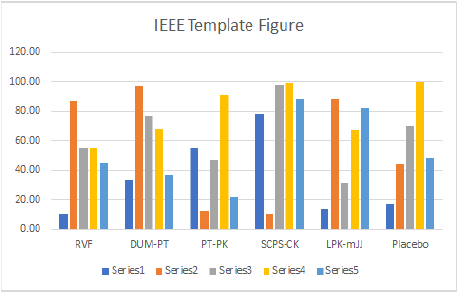
\includegraphics[width=18.5pc]{fig1.png}}
\caption{This is a sample of a figure caption.}
\end{figure}

\section{MATH}

Use either the Microsoft Equation Editor or the MathType plugin, which can be obtained from {https://store.wiris.com/en/products/mathtype/download}. For help with formatting and placing equations, refer to the {\it IEEE Editing Math Guide} at {http://journals.ieeeauthorcenter.ieee.org/wp-content/\break uploads/sites/7/Editing-Mathematics.pdf} and the {\it IEEE MathType Tutorial for Microsoft Word Users} at {http://journals.ieeeauthorcenter.ieee.org/wp-content/uploads/sites/7/IEEE-Math-Typesetting-Guide-for-MS-Word-Users.pdf}.


\subsection{Equations}

Number equations consecutively with equation numbers in parentheses flush with the right margin of the column, as in (1). First use the equation editor to create the equation. Then select the ``Equation'' markup style. Press the tab key and write the equation number in parentheses. To make your equations more compact, you may use the solidus ( / ), the exp function, or appropriate exponents. Use parentheses to avoid ambiguities in denominators. Punctuate equations when they are part of a sentence, as in
\begin{equation}
B_p+H_2=40.
\end{equation}

Be sure that the symbols in your equation have been defined before the equation appears or immediately following. Italicize symbols (T might refer to temperature, but $T$ is the unit tesla). When referring to an equation or formula, use simply ``(1),'' not ``Eq. (1)'' or ``equation (1),'' except at the beginning of a sentence: ``Equation (1) is ... .''

\begin{table}
\caption{This is a Sample of a Table Title}
\label{table}
\tablefont
\begin{tabular*}{20pc}{@{}c@{}}
\hline
\centerline{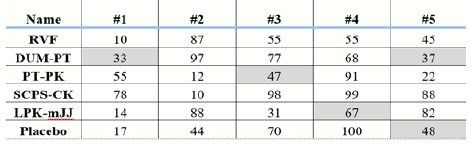
\includegraphics[width=18.5pc]{figtbl1.png}}\\
\hline
\end{tabular*}
\label{tab1}
\end{table}


\section{GUIDELINES FOR GRAPHICS PREPARATION AND SUBMISSION}

\subsection{Types of Graphics}

The following list outlines the different types of graphics published in IEEE journals. They are categorized based on their construction, and use of color / shades of gray:

\begin{enumerate}
\def\labelenumi{\arabic{enumi})}
\item
  \textbf{Color/Grayscale Figures}\\
  Figures that are meant to appear in color, or shades of black/gray. Such figures may include photographs, illustrations, multicolor graphs, and flowcharts.
\item
  \textbf{Line Art Figures}\\
  Figures that are composed of only black lines and shapes. These figures should have no shades or half-tones of gray, only black and white.
\item
  \textbf{Tables}\\
  Data charts which are typically black and white, but sometimes include color.
\end{enumerate}

\subsection{Multipart Figures}

These are figures compiled of more than one sub-figure presented side-by-side or stacked. If a multipart figure is made up of multiple figure types (one part is line art, and another is grayscale or color), the figure should meet the stricter guidelines.

\subsection{File Formats for Graphics}

Format and save your graphics using a suitable graphics processing program that will allow you to create the images as PostScript (PS), Encapsulated PostScript (.EPS), Tagged Image File Format (.TIFF), Portable Document Format (.PDF), JPEG, or Portable Network Graphics (.PNG). These programs can re-size them and adjust the resolution settings. If you created your source files in one of the following programs you will be able to submit the graphics without converting to a PS, EPS, TIFF, PDF, or PNG file: Microsoft Word, Microsoft PowerPoint, or Microsoft Excel. Though it is not required, it is strongly recommended that these files be saved in PDF format rather than DOC, XLS, or PPT. Doing so will protect your figures from common font and arrow stroke issues that occur when working on the files across multiple platforms. When submitting your final files, your graphics should all be submitted individually in one of these formats along with the manuscript.

\subsection{Sizing of Graphics}

Most charts, graphs, and tables are one column wide (3.5 inches / 88 mm / 21 picas) or page wide (7.16 inches / 181 millimeters / 43 picas). The maximum depth a graphic can be is 8.5 inches (216 millimeters / 54 picas). When choosing the depth of a graphic, please allow space for a caption. Figures can be sized between column and page widths if the author chooses, however, it is recommended that figures not be sized less than column width unless when necessary.

The final printed size of author photographs is exactly 1 in wide by 1.25 in tall (25.4 mm x 31.75 mm / 6 picas x 7.5 picas). Author photos printed in editorials measure 1.59 in wide by 2 in tall (40 mm x 50 mm / 9.5 picas x 12 picas).

\subsection{Resolution}

The proper resolution of your figures will depend on the type of figure it is as defined in the ``Types of Figures'' section. Author photographs, color, and grayscale figures should be at least 300dpi. Line art, including tables should be a minimum of 600dpi.

\subsection{Vector Art}

In order to preserve the figures' integrity across multiple computer platforms, we accept files in the following formats: .EPS/.PDF/.PS. All fonts must be embedded or text converted to outlines in order to achieve the best-quality results.

\subsection{Color Space}

The term ``color space'' refers to the entire sum of colors that can be represented within the said medium. For our purposes, the three main color spaces are grayscale, RGB (red/green/blue), and CMYK (cyan/magenta/yellow/black). RGB is generally used with on-screen graphics, whereas CMYK is used for printing purposes.

All color figures should be generated in RGB or CMYK color space. Grayscale images should be submitted in grayscale color space. Line art may be provided in grayscale OR bitmap colorspace. Note that ``bitmap colorspace'' and ``bitmap file format'' are not the same thing. When bitmap color space is selected, .TIF/.TIFF/.PNG are the recommended file formats.

\subsection{Accepted Fonts Within Figures}

When preparing your graphics, IEEE suggests that you use one of the
following Open Type fonts: Times New Roman, Helvetica, Arial, Cambria,
or Symbol. If you are supplying EPS, PS, or PDF files, all fonts must be
embedded. Some fonts may only be native to your operating system;
without the fonts embedded, parts of the graphic may be distorted or
missing.

A safe option when finalizing your figures is to strip out the fonts
before you save the files, creating ``outline'' type. This converts
fonts to artwork which will appear uniformly on any screen.

\subsection{Using Labels Within Figures}

\begin{enumerate}
\def\labelenumi{\arabic{enumi})}
\item
  \textbf{Figure Axis Labels}

  \begin{enumerate}
  \def\labelenumii{\alph{enumii})}
  \item
    Figure axis labels are often a source of confusion. Use words rather
    than symbols. As an example, write the quantity ``Magnetization'' or
    ``Magnetization \emph{M},'' not just ``\emph{M}.'' Put units in
    parentheses. Do not label axes only with units. For example, write
    ``Magnetization (A/m)'' or ``Magnetization
    (A.m$^{{-}1}$),'' not just ``A/m.'' Do not label axes with
    a ratio of quantities and units. For example, write ``Temperature
    (K),'' not ``Temperature/K.''
  \item
    Multipliers can be especially confusing. Write ``Magnetization
    (kA/m)'' or ``Magnetization (10\textsuperscript{3} A/m).'' Do not
    write ``Magnetization (A/m) X 1000'' because the reader would not
    know whether the top axis label means 16000 A/m or 0.016 A/m. Figure
    labels should be legible, approximately 8- to 10-point type.
  \end{enumerate}
\item
  \textbf{Subfigure Labels in Multipart Figures and\break Tables}

  Multipart figures should be combined and labeled before final submission. Labels should appear centered below each subfigure in 8-point Times New Roman font in the format of (a), (b) and (c).
\end{enumerate}\vspace*{-.5pc} 

\subsection{Referencing a Figure or Table Within Your Article}

When referencing your figures and tables within your article, use the abbreviation ``Fig.'' even at the beginning of a sentence. Do not abbreviate ``Table.'' Tables should be numbered with Roman numerals.\vspace*{-.5pc}

\subsection{Submitting Your Graphics}

Because IEEE will do the final formatting of your article, all figures, figure captions, and tables can be placed at the end of your article. However, if you do place your figures within the article, they should be placed at the top of the page, closest to the first mention in the text. Figures should be submitted as individual files, separate from the manuscript in one of the file formats listed above. Place figure captions below the figures; place table headings above the tables. Do not include captions as part of the figures, or put them in ``text boxes'' linked to the figures. Also, do not place borders around the outside of your figures.\vspace*{-.5pc}

\subsection{Color Processing / Printing in IEEE Transactions, Journals, and Letters}

All IEEE Transactions, Journals, and Letters allow an author to publish color figures on IEEE \emph{Xplore} at no charge, and automatically convert them to grayscale for print versions. In most journals, figures and tables may alternatively be printed in color if an author chooses to do so. Please note that this service comes at an extra expense to the author. If you intend to have print color graphics, you will have the opportunity to indicate this in the Author Gateway and will be contacted by PubOps to confirm the charges.\vspace*{-.5pc}

\section{CONCLUSION}
A conclusion section is not required. Although a conclusion may review the main points of the article, do not replicate the abstract as the conclusion. A conclusion might elaborate on the importance of the work or suggest applications and extensions.\vspace*{-.5pc}

\section*{APPENDIX}

Appendixes, if needed, appear before the acknowledgment.

\section*{ACKNOWLEDGMENT}

The preferred spelling of the word ``acknowledgment'' in American English is without an ``e'' after the ``g.'' Use the singular heading even if you have many acknowledgments. Avoid expressions such as ``One of us (S.B.A.) would like to thank ... .'' Instead, write ``F. A. Author thanks ... .'' In most cases, sponsor and financial support acknowledgments are placed in the unnumbered footnote on the first page, not here.

\section*{REFERENCES AND FOOTNOTES}

\subsection{References}

References need not be cited in text. When they are, they appear on the line, in square brackets, inside the punctuation. Multiple references are each numbered with separate brackets. When citing a section in a book, please give the relevant page numbers. In text, refer simply to the reference number. Do not use ``Ref.'' or ``reference'' except at the beginning of a sentence: ``Reference {[}3{]} shows ... .'' Please do not use automatic endnotes in \emph{Word}, rather, type the reference list at the end of the paper using the ``References'' style.

Reference numbers are set flush left and form a column of their own, hanging out beyond the body of the reference. The reference numbers are on the line, enclosed in square brackets. In all references, the given name of the author or editor is abbreviated to the initial only and precedes the last name. Use them all; use \emph{et al}. only if names are not given or if there are more than 6 authors. Use commas around Jr., Sr., and III in names. Abbreviate conference titles. When citing IEEE Transactions, provide the issue number, page range, volume number, month if available, and year. When referencing a patent, provide the day and the month of issue, or application. References may not include all information; please obtain and include relevant information. Do not combine references. There must be only one reference with each number. If there is a URL included with the reference, it can be included at the end of the reference.

Other than books, capitalize only the first word in an article title, except for proper nouns and element symbols. For articles published in translation journals, please give the English citation first, followed by the original foreign-language citation. See the end of this document for formats and examples of common references. For a complete discussion of references and their formats, see the \emph{IEEE Editorial Style Manual} \emph{for Authors} at {{https://journals.ieeeauthorcenter.ieee.org/create-your-ieee-journal-article/create-the-text-of-your-article/ieee-editorial-style-manual/}}.

\subsection{Footnotes}

Number footnotes separately in superscripts (Insert \textbar{}Footnote).\footnote{It is recommended that footnotes be avoided (except for the unnumbered footnote with the receipt date on the first page). Instead, try to integrate the footnote information into the text.} Place the actual footnote at the bottom of the column in which it is cited; do not put footnotes in the reference list (endnotes). Use letters for table footnotes (see Table I).

\section{SUBMITTING YOUR ARTICLE FOR REVIEW}

\subsection{Review Stage Using ScholarOne Manuscripts}

Contributions to the Transactions, Journals, and Letters may be submitted electronically on IEEE's online manuscript submission and peer-review system, ScholarOne Manuscripts. You can get help choosing the correct publication for your manuscript as well as find their corresponding ScholarOne Manuscripts peer review site using the tools listed at {{http://www.ieee.org/publications\_standards/\break publications/authors/authors\_submission.html}} Once you have chosen your publication and navigated to the ScholarOne site, check first to see if you have an existing account. If there is none, please create a new account. After logging in, go to your Author Center and click ``Start New Submission.''

Along with other information, you will be asked to select the manuscript type from the journal's pre-determined list of options. Depending on the journal, there are various steps to the submission process; please make sure to carefully answer all of the submission questions presented to you. At the end of each step you must click ``Save and Continue''; just uploading the paper is not sufficient. After the last step, you should see a confirmation that the submission is complete. You should also receive an e-mail confirmation. For inquiries regarding the submission of your paper on ScholarOne Manuscripts, please contact oprs-support@ieee.org or call +1 732 465 5861.

ScholarOne Manuscripts will accept files for review in various formats. There is a ``Journal Home'' link on the log-in page of each ScholarOne Manuscripts site that will bring you to the journal's homepage with their detailed requirements; please check these guidelines for your particular journal before you submit.

\subsection{Final Stage Using ScholarOne Manuscripts}

Upon acceptance, you will receive an email with specific instructions regarding the submission of your final files. To avoid any delays in publication, please be sure to follow these instructions. Final submissions should include source files of your accepted manuscript, high quality graphic files (if not embedded in your source file), and a formatted pdf file. The accepted version of your manuscript will also be sent to the IEEE publication teams for a comparison to the final files to ensure no significant or unauthorized changes were made after acceptance. If you have any questions regarding the final submission process, please contact the administrative contact for the journal.

When submitting your final files on a hybrid OA journal you will have the opportunity to designate your article as ``open access'' if you agree to pay the IEEE open access fee. Please select the appropriate choice. Immediately after you have submitted your final files through ScholarOne Manuscripts you will be automatically redirected to the IEEE electronic copyright form wizard. Please complete the copyright at that time to avoid publication delays.

\subsection{Copyright Form}

Authors must submit an electronic IEEE Copyright Form (eCF) upon submitting their final manuscript files.~You can access the eCF system through your manuscript submission system or through the Author Gateway. You are responsible for obtaining any necessary approvals and/or security clearances. For additional information on intellectual property rights, visit the IEEE Intellectual Property Rights department web page at {{https://www.ieee.org/publications/rights/index.html}}

\section{IEEE GUIDELINES AND POLICIES}

A full overview of IEEE publishing guidelines and policies can be found
at {{https://journals.ieeeauthorcenter.ieee.org/become-an-ieee-journal-author/publishing-ethics/guidelines-and-policies/}}. They are designed to help authors understand and navigate the publishi process successfully. Learn more about IEEE's fundamental publishing guidelines and principles, submission and peer review policies, post-publication policies, and guidelines on advertising, accessibility, and data privacy.

\bibsection*{REFERENCES}

\bibsection*{\itshape Basic format for periodicals:}\vspace*{-12pt}
\def\refname{}
\begin{thebibliography}{[34]}
\item[]  J. K. Author, ``Name of paper,'' \emph{Abbrev. Title of Periodical}, vol. x, no. x, pp. xxx--xxx, Abbrev. Month, year, doi: \href{https://dx.doi.org/10.1109.XXX.1234567}{10.1109.XXX.1234567}.
\end{thebibliography}

\bibsection*{\itshape Periodicals using article numbers:}
\def\refname{}
\begin{thebibliography}{[34]}\vspace*{-12pt}
\item[] J. K. Author, ``Name of paper,'' \emph{Abbrev. Title of Periodical}, vol. x, no. x, Abbrev. Month, year, Art. no. xxxxx, doi: \href{https://dx.doi.org/10.1109.XXX.1234567}{10.1109.XXX.1234567}.
\end{thebibliography}

\bibsection*{\itshape Examples:}\vspace*{-12pt}
\begin{thebibliography}{[34]}
\setcounter{enumiv}{0}
\bibitem{bib1}J. U. Duncombe, ``Infrared navigation---Part I: An assessment of feasibility,'' IEEE Trans. Electron Devices, vol. ED-11, no. 1, pp. 34--39, Jan. 1959, doi: \href{https://dx.doi.org/10.1109/TED.2016.2628402}{10.1109/TED.2016.2628402}.
\bibitem{bib2}E. P. Wigner, ``Theory of traveling-wave optical laser,'' \emph{Phys. Rev}., vol. 134, pp. A635--A646, Dec. 1965.
\bibitem{bib3}P. Kopyt \emph{et al., ``}Electric properties of graphene-based conductive layers from DC up to terahertz range,'' \emph{IEEE THz Sci. Technol.,} to be published, doi: \href{https://dx.doi.org/10.1109/TTHZ.2016.2544142}{10.1109/TTHZ.2016.2544142}. \emph{(Note: If a paper is still to be published, but is available in early access, please follow ref {[}5{]}.)}
\bibitem{bib4}R. Fardel, M. Nagel, F. Nuesch, T. Lippert, and A. Wokaun,  ``Fabrication of organic light emitting diode pixels by laser-assisted forward transfer,'' \emph{Appl. Phys. Lett.}, vol. 91, no. 6, Aug. 2007, Art. no. 061103.~
\bibitem{bib5}D. Comite and N. Pierdicca, ``Decorrelation of the near-specular land scattering in bistatic radar systems,'' \emph{IEEE Trans. Geosci. Remote Sens.}, early access, doi: \href{https://dx.doi.org/10.1109/TGRS.2021.3072864}{10.1109/TGRS.2021.3072864}. (\emph{Note: This format is used for articles in early access. The doi must be included.})
\bibitem{bib6}H. V. Habi and H. Messer, ``Recurrent neural network for rain estimation using commercial microwave links,'' \emph{IEEE Trans. Geosci. Remote Sens.}, vol. 59, no. 5, pp. 3672--3681, May 2021. {[}Online{]}. Available: https://ieeexplore.ieee.org/document/9153027
\end{thebibliography}


\bibsection*{\itshape Basic format for books:}\vspace*{-12pt}
\begin{thebibliography}{[34]}
\item[] J. K. Author, ``Title of chapter in the book,'' in \emph{Title of Published Book, x}th ed. City of Publisher, (only U.S. State), Country: Abbrev. of Publisher, year, ch. x, sec. \emph{x}, pp. xxx--xxx\emph{.}
\end{thebibliography}


\bibsection*{\itshape Examples:}\vspace*{-12pt}
\begin{thebibliography}{[34]}
\setcounter{enumiv}{6}
\bibitem{bib7}G. O. Young, ``Synthetic structure of industrial plastics,'' in \emph{Plastics,} 2nd ed., vol. 3, J. Peters, Ed. New York, NY, USA: McGraw-Hill, 1964, pp. 15--64.
\bibitem{bib8}W.-K. Chen, \emph{Linear Networks and Systems.} Belmont, CA, USA: Wadsworth, 1993, pp. 123--135.
\bibitem{bib9}Philip B. Kurland and Ralph Lerner, eds., \emph{The Founders' Constitution.} Chicago, IL, USA: Univ. of Chicago Press, 1987, Accessed on: Feb. 28, 2010, {[}Online{]}. Available: http://press-pubs.uchicago.edu/founders/
\end{thebibliography}

\bibsection*{\itshape Basic format for handbooks:}\vspace*{-12pt}
\begin{thebibliography}{[34A]}
\item[]  \emph{Name of Manual/Handbook, x} ed., Abbrev. Name of Co., City of Co., Abbrev. State, Country, year, pp. xxx--xxx.
\end{thebibliography}

\bibsection*{\itshape Examples:}\vspace*{-12pt}
\begin{thebibliography}{[31d]}
\setcounter{enumiv}{9}
\bibitem{bib10}\emph{Transmission Systems for Communications}, 3rd ed., Western Electric Co., Winston-Salem, NC, USA, 1985, pp. 44--60.
\bibitem{bib11}\emph{Motorola Semiconductor Data Manual}, Motorola Semiconductor Products Inc., Phoenix, AZ, USA, 1989.
\bibitem{bib12}R. J. Hijmans and J. van Etten, ``Raster: Geographic analysis and modeling with raster data,'' R Package Version 2.0-12, Jan. 12, 2012. {[}Online{]}. Available: \emph{http://CRAN.R-project.org/package=raster}
\end{thebibliography}

\bibsection*{\itshape Basic format for reports:}\vspace*{-12pt}

\begin{thebibliography}{[31d]}
\item[]  J. K. Author, ``Title of report,'' Abbrev. Name of Co., City of Co., Abbrev. State, Country, Rep. xxx, year.
\end{thebibliography}

\bibsection*{\itshape Example:}\vspace*{-12pt}
\begin{thebibliography}{[31d]}
\setcounter{enumiv}{12}
\bibitem{bib13}E. E. Reber, R. L. Michell, and C. J. Carter, ``Oxygen absorption in the earth's atmosphere,'' Aerospace Corp., Los Angeles, CA, USA, Tech. Rep. TR-0200 (4230-46)-3, Nov. 1988.
\end{thebibliography}

\bibsection*{\itshape Basic format for conference proceedings:}\vspace*{-12pt}
\begin{thebibliography}{[31d]}
\item[] J. K. Author, ``Title of paper,'' in \emph{Abbreviated Name of Conf.}, City of Conf., Abbrev. State (if given), Country, year, pp. xxxxxx\emph{.}
\end{thebibliography}

\bibsection*{\itshape Examples:}\vspace*{-12pt}
\begin{thebibliography}{[31d]}
\setcounter{enumiv}{13}
\bibitem{bib14}D. B. Payne and J. R. Stern, ``Wavelength-switched passively coupled single-mode optical network,'' in \emph{Proc. IOOC-ECOC,} Boston, MA, USA, 1985, pp. 585--590.
\bibitem{bib15}D. Ebehard and E. Voges, ``Digital single sideband detection for interferometric sensors,'' presented at the 2nd Int. Conf. Optical Fiber Sensors\emph{,} Stuttgart, Germany, Jan. 2-5, 1984.
\bibitem{bib16}PROCESS Corporation, Boston, MA, USA. Intranets: Internet technologies deployed behind the firewall for corporate productivity. Presented at INET96 Annual Meeting. {[}Online{]}. Available: http://home.process.com/Intranets/wp2.htp
\end{thebibliography}

\bibsection*{\itshape Basic format for electronic documents (when available online):}\vspace*{-12pt}
\begin{thebibliography}{[31d]}
\item[] Issuing Organization. (year, month day). \emph{Title}. {[}Type of medium{]}. Available: site/path/file
\end{thebibliography}

\bibsection*{\itshape Example:}\vspace*{-12pt}
\begin{thebibliography}{[31d]}
\setcounter{enumiv}{16}
\bibitem{bib17}U.S. House. 102nd Congress, 1st Session. (1991, Jan. 11). \emph{H. Con. Res. 1, Sense of the Congress on Approval of Military Action}. {[}Online{]}. Available: LEXIS Library: GENFED File: BILLS
\end{thebibliography}

\bibsection*{\itshape Basic format for patents:}\vspace*{-12pt}
\begin{thebibliography}{[31d]}
\item[] J. K. Author, ``Title of patent,'' U.S. Patent \emph{x xxx xxx}, Abbrev. Month, day, year.
\end{thebibliography}

\bibsection*{\itshape Example:}\vspace*{-12pt}
\begin{thebibliography}{[31d]}
\setcounter{enumiv}{17}
\bibitem{bib18}   G. Brandli and M. Dick, ``Alternating current fed power supply,'' U.S. Patent 4 084 217, Nov. 4, 1978.
\end{thebibliography}

\bibsection*{\itshape Basic format for theses (M.S.) and dissertations (Ph.D.):}\vspace*{-12pt}
\begin{thebibliography}{[31d]}
\item[] J. K. Author, ``Title of thesis,'' M.S. thesis, Abbrev. Dept., Abbrev. Univ., City of Univ., Abbrev. State, year.
\item[] J. K. Author, ``Title of dissertation,'' Ph.D. dissertation, Abbrev. Dept., Abbrev. Univ., City of Univ., Abbrev. State, year.
\end{thebibliography}

\bibsection*{\itshape Examples:}\vspace*{-12pt}
\begin{thebibliography}{[31d]}
\setcounter{enumiv}{18}
\bibitem{bib19}J. O. Williams, ``Narrow-band analyzer,'' Ph.D. dissertation, Dept. Elect. Eng., Harvard Univ., Cambridge, MA, USA, 1993.
\bibitem{bib20}N. Kawasaki, ``Parametric study of thermal and chemical nonequilibrium nozzle flow,'' M.S. thesis, Dept. Electron. Eng., Osaka Univ., Osaka, Japan, 1993.
\end{thebibliography}

\bibsection*{\itshape Basic format for the most common types of unpublished references:}\vspace*{-12pt}
\begin{thebibliography}{[31d]}
\item[] J. K. Author, private communication, Abbrev. Month, year.
\item[] J. K. Author, ``Title of paper,'' unpublished.
\item[] J. K. Author, ``Title of paper,'' to be published.
\end{thebibliography}

\bibsection*{\itshape Examples:}\vspace*{-12pt}

\begin{thebibliography}{[31d]}
\setcounter{enumiv}{20}
\bibitem{bib21}A. Harrison, private communication, May 1995.
\bibitem{bib22}B. Smith, ``An approach to graphs of linear forms,'' 2014, \emph{arXiv:2105.02824}.
\bibitem{bib23}A. Brahms, ``Representation error for real numbers in binary computer arithmetic,'' IEEE Computer Group Repository, Paper R-67-85.
\end{thebibliography}


\bibsection*{\itshape Basic formats for standards:}\vspace*{-12pt}
\begin{thebibliography}{[31d]}
\item[a)]\emph{Title of Standard}, Standard number, date.
\item[b)]\emph{Title of Standard}, Standard number, Corporate author, location, date.
\end{thebibliography}


\bibsection*{\itshape Examples:}\vspace*{-12pt}
\begin{thebibliography}{[31d]}
\setcounter{enumiv}{23}

\bibitem{bib24}IEEE Criteria for Class IE Electric Systems, IEEE Standard 308, 1969.
\bibitem{bib25}Letter Symbols for Quantities, ANSI Standard Y10.5-1968.
\end{thebibliography}


\biographysection

\begin{IEEEbiography}{First A. Author}{\space}(Fellow, IEEE) and all authors may include biographies if the publication allows. Biographies are often not included in conference-related papers. Please check the Information for Authors to confirm. Author photos should be current, professional images of the head and shoulders. The first paragraph may contain a place and/or date of birth (list place, then date). Next, the author's educational background is listed. The degrees should be listed with the type of degree in what field, which institution, city, state, and country, and year the degree was earned. The author's major field of study should be lowercase.

The second paragraph uses the preferred third person pronoun (he, she, they, etc.) and not the author's last name. It lists military and work experience, including summer and fellowship jobs. Job titles are capitalized. The current job must have a location; previous positions may be listed without one. Information concerning previous publications may be included. The format for listing publishers of a book within the biography is: \emph{Title of Book} (publisher name, year) similar to a reference. Current and previous research interests end the paragraph.

The third paragraph begins with the author's preferred title and last name (e.g., Dr. Smith, Prof. Jones, Mr. Kajor, Ms. Hunter, Mx. Riley). List any memberships in professional societies other than the IEEE. Finally, list any awards and work for IEEE committees and publications.
\end{IEEEbiography}

\begin{IEEEbiography}{Second B. Author}{\space}photograph and biography not available at the time of publication.
\end{IEEEbiography}

\begin{IEEEbiography}{Third C. Author, Jr.} (Member, IEEE), photograph and biography not available at the time of publication.
\end{IEEEbiography}
\end{document}
